%%%%%%%%%%%%%%%%%%%%%%%%%%%%%%%%%%%%%%%%%%%%%%%%%%%%%%%%%%
%
% eXascale Infolab thesis template -- Bachelor and Masters
% version 1.1, Oct 2019
%
%%%%%%%%%%%%%%%%%%%%%%%%%%%%%%%%%%%%%%%%%%%%%%%%%%%%%%%%%%
%
% Based on:
% Masters/Doctoral Thesis
% LaTeX Template Version 2.5 (27/8/17)
% http://www.LaTeXTemplates.com
% CC BY-NC-SA 3.0 (http://creativecommons.org/licenses/by-nc-sa/3.0/)
%
%%%%%%%%%%%%%%%%%%%%%%%%%%%%%%%%%%%%%%%%%

\documentclass[11pt,english,singlespacing,headsepline,consistentlayout]{structure/XI_thesis}

%----------------------------------------------------------------------------------------
%	LATEX PACKAGES
%----------------------------------------------------------------------------------------

%%%%%%%%%%%%%%%%%%%%%%%%%%% DO NOT EDIT
\usepackage[utf8]{inputenc} % Required for inputting international characters
\usepackage[T1]{fontenc} % Output font encoding for international characters
\usepackage{mathpazo} % Use the Palatino font by default
\usepackage[backend=bibtex,style=authoryear,natbib=true]{biblatex} % Use the bibtex backend with the authoryear citation style (which resembles APA)
\usepackage[autostyle=true]{csquotes} % Required to generate language-dependent quotes in the bibliography
\usepackage{booktabs}       % professional-quality tables
\usepackage{array}          % custom sizes for table columns
\usepackage{amssymb}        % extended blackboard math symbols
\usepackage{amsmath}        % complete AMS math package
% \usepackage[english]{babel} % spelling / syllabification
\usepackage{algorithm}      % pseudocode float
\usepackage[noend]{algpseudocode}  % pseudocode macros
\usepackage{graphicx}       % include graphics
\usepackage{epstopdf}       % vectorial graphics
\usepackage{subcaption}     % sub captions
\usepackage{url}            % URLs
%%%%%%%%%%%%%%%%%%%%%%%%%%% DO NOT EDIT - end

% Define path and extensions for your graphics
\graphicspath{{figures/}}%{{../jpeg/} [...]}
\DeclareGraphicsExtensions{.pdf,.jpg,.jpeg,.png,eps}


%% User packages
% \usepackage{add here}
% Include your package settings in `structure/settings.tex`



% Load package settings
% !TEX root = ../main.tex

%----------------------------------------------------------------------------------------
% PACKAGE CONFIGURATIONS
%----------------------------------------------------------------------------------------

% Filename of the bibliography
\addbibresource{structure/zotero.bib}

% Margin settings
\geometry{
  paper=a4paper, % Paper format
  inner=2.5cm, % Inner margin
  outer=3.8cm, % Outer margin
  bindingoffset=.5cm, % Binding offset
  top=1.5cm, % Top margin
  bottom=1.5cm, % Bottom margin
  %showframe, % Uncomment to show how the type block is set on the page
}

% Figures location
\graphicspath{{figures/}}
\DeclareGraphicsExtensions{.pdf,.png,.jpg,.jpeg,.eps,.ps}

% Load custom thesis information (remember to fill in)
% !TEX root = ../main.tex

%----------------------------------------------------------------------------------------
% THESIS INFORMATION
%----------------------------------------------------------------------------------------

\thesistitle{Binary Tree Models for Reinforcement Learning Continuous Control} % Your thesis title, this is used in the title and abstract, print it elsewhere with \ttitle
\supervisor{Prof. Dr. Philippe Cudré-Mauroux} % Your supervisor's name, this is used in the title page, print it elsewhere with \supname
\secondsupervisior{Dr. Giuseppe Cuccu}
\degree{Bachelor} % Your degree name, this is used in the title page and abstract, print it elsewhere with \degreename
\author{David Gauch} % Your name, this is used in the title page and abstract, print it elsewhere with \authorname
\addresses{Bd de Pérolles 90} % Your address, this is not currently used anywhere in the template, print it elsewhere with \addressname

\subject{Computer Science} % Your subject area, this is not currently used anywhere in the template, print it elsewhere with \subjectname
\keywords{reinforcement learning, black-box optimization, binary trees, architecture search} % Keywords for your thesis, this is not currently used anywhere in the template, print it elsewhere with \keywordnames
\university{\href{http://www.unifr.ch}{University of Fribourg}} % Your university's name and URL, this is used in the title page and abstract, print it elsewhere with \univname
\department{\href{https://www3.unifr.ch/inf/fr/}{Department of Informatics}} % Your department's name and URL, this is used in the title page and abstract, print it elsewhere with \deptname
\group{\href{https://www3.unifr.ch/inf/en/exascale-infolab.html}{eXascale Infolab}} % Your research group's name and URL, this is used in the title page, print it elsewhere with \groupname
\faculty{\href{https://www3.unifr.ch/scimed/fr/}{Faculty of Science and Medicine}} % Your faculty's name and URL, this is used in the title page and abstract, print it elsewhere with \facname

% Set title, author and keywords on the compiled PDF
\AtBeginDocument{
  \hypersetup{pdftitle=\ttitle} % Set the PDF's title to your title
  \hypersetup{pdfauthor=\authorname} % Set the PDF's author to your name
  \hypersetup{pdfkeywords=\keywordnames} % Set the PDF's keywords to your keywords
}

%----------------------------------------------------------------------------------------
\begin{document}
\frontmatter
\pagestyle{plain}
% Title page definition
% !TEX root = ../main.tex

%----------------------------------------------------------------------------------------
% TITLE PAGE
%----------------------------------------------------------------------------------------

\begin{titlepage}
\begin{center}

%\includegraphics[width=15cm]{logos/xi_logos}
%\vspace*{.06\textheight}
%\\

\begin{figure}
  \centering
    \includegraphics[width=.17\textwidth]{logos/unifr_logo}
  \hfill
    \includegraphics[width=.4\textwidth]{logos/xi_logo}
  \vspace{30mm}
\end{figure}

{\scshape\LARGE \univname\par}\vspace{1.5cm} % University name
\textsc{\Large Bachelor Thesis}\\[0.5cm] % Thesis type
\HRule \\[0.4cm] % Horizontal line
{\huge \bfseries \ttitle\par}\vspace{0.4cm} % Thesis title
\HRule \\[1.5cm] % Horizontal line

\begin{minipage}[t]{0.4\textwidth}
\begin{flushleft} \large
\emph{Author:}\\
\href{mailto:david.gauch@unifr.ch}{\authorname} % Author name - remove the \href bracket to remove the link
\end{flushleft}
\end{minipage}
\begin{minipage}[t]{0.4\textwidth}
\begin{flushright} \large
\emph{Supervisor:} \\
\href{https://exascale.info/phil}{\supname} % Supervisor name - remove the \href bracket to remove the links
\\
\href{https://exascale.info/giuse}{\secondsupname}
\end{flushright}
\end{minipage}\\[1cm]

May 10, 2023 % date of the official defense
\vspace*{.06\textheight}

%\large \textit{A thesis submitted in fulfillment of the requirements\\ for the degree of \degreename}\textit{ in the}\\[0.3cm] % University requirement text
\groupname\\\deptname\\ % Research group name and department name
\vfill

\footnotesize{ Boulevard de Pérolles 90 ~~$\bullet$~~ 1700~Fribourg ~~$\bullet$~~ Switzerland
            \\
            phone +41~(26)~300~84~65 ~~$\bullet$~~ \textsf{diuf-secr@unifr.ch} ~~$\bullet$~~ \textsf{www3.unifr.ch/inf}
            }


\end{center}
\end{titlepage}

% Include declaration page -- not necessary for Bachelor and Masters
% \input{declaration.tex}
\cleardoublepage

%----------------------------------------------------------------------------------------
%	QUOTATION PAGE
%----------------------------------------------------------------------------------------
% Include only in the final submission, after the defense and all required corrections

%\vspace*{0.2\textheight}
%\noindent\enquote{\itshape Quote here}\bigbreak


%----------------------------------------------------------------------------------------
%   ABSTRACT PAGE
%----------------------------------------------------------------------------------------
\begin{abstract}
\addchaptertocentry{\abstractname} % Add the abstract to the table of contents
% !TEX root = ../main.tex

Neural networks are widely used for machine learning due to the large amount of data available, especially in deep learning. However, when it comes to solving non-continuous control tasks in the field of reinforcement learning, neural networks can be counterintuitive since they are continuous. To address this issue, this project explores the hypothesis that binary trees, as discontinuous models, could have an advantage in solving these tasks. To further develop this model, the project introduces an insertion strategy that allows the tree to grow dynamically when tasks become too complex for its current structure. This technique should be a first step toward architecture search for binary trees. The approach has been tested on various benchmarks and the results are promising, indicating that a growing binary tree could be an efficient model for solving many control tasks. The project provides valuable insights into the use of the binary tree as an alternative model for reinforcement learning and highlights the potential benefits of using dynamic structures such as growing the trees for efficient and effective learning.
\vfill
\begin{center}
\textbf{Keywords:}~\keywordnames
\end{center}
\end{abstract}


%----------------------------------------------------------------------------------------
%	LIST OF CONTENTS/FIGURES/TABLES + TRANSITION PAGES
%----------------------------------------------------------------------------------------
\hypersetup{linkcolor=black}
\tableofcontents % Prints the main table of contents
\listoffigures % Prints the list of figures
\mainmatter % Begin numeric (1,2,3...) page numbering
\pagestyle{thesis} % Return the page headers back to the "thesis" style


%----------------------------------------------------------------------------------------
%	THESIS CONTENT - CHAPTERS
%----------------------------------------------------------------------------------------

% Include here the chapters of the thesis
% Comment/uncomment the lines to find bugs and compile faster during writing
% \include{structure/template_intro} % comment this out
% !TEX root = ../main.tex

\chapter{Introduction}
\label{ch:introduction}

\section{Reinforcement learning}
Reinforcement learning is a type of machine learning that focuses on training agents to make decisions in dynamic environments in order to maximize a reward signal. It is distinct from other paradigms such as supervised learning, which uses labeled data to predict outputs for unseen data, and unsupervised learning, which seeks to find patterns in unlabeled data. In addition to being a problem that can be addressed with specific solution methods, reinforcement learning is also the field of study that examines this problem and its potential solutions. Overall, the goal of reinforcement learning is to teach agents to make optimal decisions in order to achieve a desired outcome or reward.(\cite{sutton_reinforcement_2018}).

\vspace{5mm}

Classical reinforcement learning involves the interaction between two main components: an environment and an agent. The environment is represented by a current state that provides information about the "world" in which the agent is located, and the agent is the individual who performs actions within this environment. In each interaction, the agent receives observations based on the current state of the environment and selects an action to take. This action is then transmitted to the environment, which updates its internal state and provides feedback to the agent in the form of observations and a reward. The reward signal indicates whether the action was suitable for completing the task, while the observations provide an overview of the updated environment. Figure~\ref{fig:RL_main_loop} illustrates one timestep of interaction between the agent and the environment.
\begin{figure}[!ht]
\centering
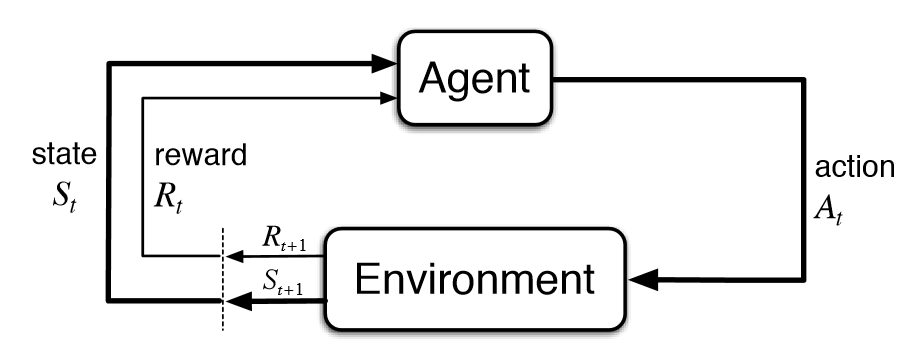
\includegraphics[width=.6\textwidth]{RL_main_loop}
\caption[Main interaction of the agent and the environment in reinforcement learning]{
  \textbf{Main interaction of the agent and the environment in reinforcement learning.}
  At the beginning (timestep $t$) the agent gets the observation $S_t$ and the reward $R_t$ from the environment. The agent performs then action $A_t$ and sends it to the environment. The environment changes its state and returns a new observation $S_{t+1}$ and a new reward $R_{t+1}$.
  
 }
\label{fig:RL_main_loop}
\end{figure}

\vspace{5mm}

In reinforcement learning, the policy is a key element of the framework that determines the actions an agent should take in different states of the environment. The policy is represented by a mapping from states to actions, and it can be either deterministic or stochastic. Deterministic policies specify a single action to take in each state, while stochastic policies specify probabilities for different actions to occur. The reward an agent receives depends on the chosen policy, and the sequence of states reached by the agent is called a Markov chain. This mathematical concept models systems that change over time in a way that depends only on the current state and not on the history of past states.(\cite{sutton_reinforcement_2018}).

The value function is a key concept in reinforcement learning that allows us to evaluate the effectiveness of different policies.$V_{\pi}(s)$ defines the expected total reward that an agent can expect to receive by following the policy $\pi$, starting from state $s$. One way to compute the value function is using the Bellman equation, which expresses the value of a state in terms of the values of its successors(\cite{barron_bellman_1989}). However, the Bellman equation does not have a closed-form solution, which makes it challenging to compute the value function in practice.
The value function can be used to define an optimal policy, which is the policy that is expected to maximize the reward over time. Another way to analyze policies is using the Q-function.$Q_{\pi}(s, a)$ is defined as the expected total reward acquired by the agent following policy $\pi$ starting from state $s$ and taking action $a$. The Q-function can be related to the value function through the equation $V_{\pi}(s) = Q_{\pi}(s, \pi(s))$. A common method for finding the optimal Q-function is Q-learning, which is an iterative process that updates the Q-function based on experience (\cite{watkins_q-learning_1992}). 

\vspace{5mm}

Reinforcement learning is well-suited for autonomous systems that learn to achieve a desired outcome through trial and error. However, this paradigm presents a unique challenge that is not encountered in supervised or unsupervised learning: balancing exploitation and exploration. Exploitation refers to the process of repeating actions that have resulted in positive rewards in the past, in order to maximize the cumulative reward. On the other hand, exploration involves trying new actions in order to potentially discover higher rewards and avoid getting stuck in a local optimum. Finding the right balance between these two approaches is crucial for the success of the learning process.

While reinforcement learning has been effective in solving a range of tasks, it has also encountered challenges in real-world applications (\cite{zhu_ingredients_2020}). In this thesis, however, the paradigm is sufficient for addressing the desired tasks. Overall, reinforcement learning offers a powerful tool for training agents to make decisions in dynamic environments and optimize for a given reward signal.

\section{Black-Box Optmization}

In mathematics, optimization refers to the process of finding the maximum or minimum value of an objective function. Neural networks, for example, try to find the best weights for approximating an underlying function using techniques such as backpropagation and gradient descent. However, these techniques require knowledge of the derivative of the function, which may not always be available or may be too complex to compute (\cite{schaul_studies_nodate}). Black-box optimization is a method that does not rely on any assumptions about the function or its properties, and can be used to optimize any function approximator. It is based on a feedback score similar to reinforcement learning, and the parameter set is improved based on this score (\cite{anderson_introduction_1995}).

Black-box optimization methods are generally less efficient than traditional techniques such as gradient descent because they do not take advantage of information about the structure of the function being optimized. This means they must explore a larger space of possible solutions, which can be time-consuming. However, black-box optimization methods can be effective in situations where the function being optimized is highly complex or has a large number of variables, and traditional methods may not be applicable. They are also flexible and can be applied to a wide range of problems without requiring any knowledge of the function being optimized

\subsection{Evolution strategies}

Evolution strategies (ES) is a class of evolutionary algorithms that is specialized for optimization of continuous variables. Inspired by natural evolution, ES is a black-box optimization algorithm that uses a process of mutation and selection to search for good solutions to a given problem. In the main loop of the algorithm, new individuals are created by mutating the parent individuals of the current generation. An individual in the context of ES refers to a specific set of parameters being optimized by the algorithm. A population is a group of individuals being considered by the algorithm at a given time, and a generation refers to one iteration of the main loop. The fitness of an individual is a measure of its performance or quality, based on the feedback score provided by the algorithm.

The main loop of the ES algorithm consists of creating new individuals from the parent individuals of the current generation, evaluating their fitness, and selecting the best-performing individuals to be the parent individuals for the next generation. This process continues until a sufficient solution is found, as determined by a stopping criterion. Algorithms differ in the number of offsprings created per generation, the number of selected individuals for the next generation, and how the mutation process is performed (\cite{salimans_evolution_2017}). Other than gradient-descent based methods, ES generates multiple individuals and by that explores different areas or paths of the optimization space independently, which can be beneficial for avoiding local optima and solving real-world problems that may require sophisticated exploration mechanisms.


\subsection{Covariance Matrix Adapation Evolution Strategy}

\section{Binary trees}

Trees are a commonly used data structure in mathematics and computer science that are composed of nodes and edges. A tree is an undirected, connected, acyclic graph, which means that it consists of a set of nodes that are connected by edges, but there are no loops or cycles in the graph. In a tree, a node that connects other nodes is called a parent node, and the nodes that are connected to it are called children nodes. The node at the top of the tree, which has no parent nodes, is called the root node, and the nodes at the bottom of the tree, which have no children, are called leaf nodes. The levels of a tree are determined by the distance from the root node, with the root node being at level 0 and the nodes connected to it being at level 1, and so on. Nodes on the same level are called sibling nodes.

Binary trees are a special type of tree in which all nodes except for the leaf nodes have at most two children nodes. These children nodes are typically referred to as the left node and the right node, respectively. An example of a binary tree is shown in Figure \ref{fig:binary_tree}.

\begin{figure}[!ht]
\centering
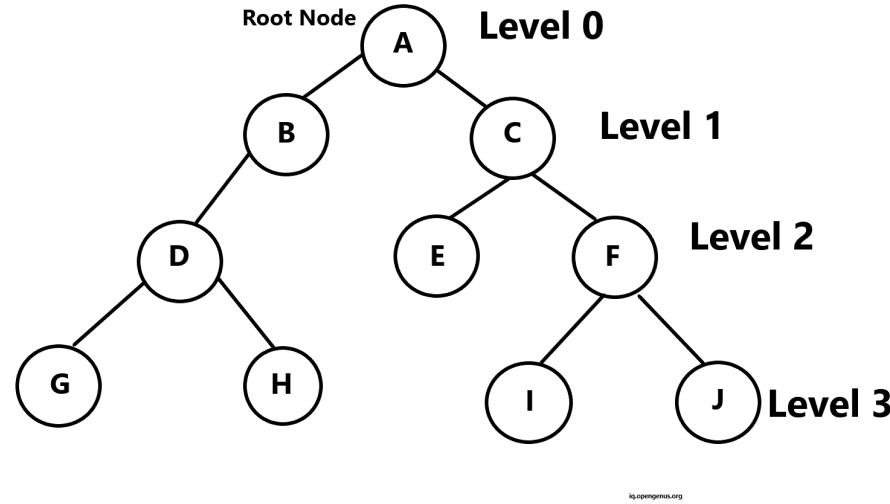
\includegraphics[width=.6\textwidth]{binary_tree}
\caption[Binary tree with letters representing the data]{
  \textbf{Binary tree with letters representing the data}
  }
\label{fig:binary_tree}
\end{figure}

\section{Open AI Gym}






% !TEX root = ../main.tex
\chapter{Method}
\label{ch:method}

\subsection{Experiment of this project}
In the context of this project, the observation is that current models are typically continuous (due to back-propagation), but many control tasks are not. An example of this is the problem of the pendulum with a fixed joint above and a loose joint below, which is swung up in a first step and then stabilized in the second step. When attempting to approximate the function that models this task, it becomes apparent that the function is not continuous. Due to the two distinct tasks involved, the agent must be able to recognize when the first task is complete and the second one begins. In the real world, there are many control problems that are not continuous.
The hypothesis is that discontinuous models would have an advantage in addressing these tasks. To test this hypothesis, multiple individuals can be evaluated in the environment (by going through the fitness function) and analyzing their performance, the number of individuals that solve the task, and other metrics. Hyperparameters also play an important role in improving the performance of individuals in the environment.

\section{Fitness}

The fitness class serves as an interface between the model and the environment. It implements the control loop at its core, through the $fit$ function.
The control loop essentially evaluates how well a set of weights performs in an environment by selecting actions, as determined by the model, and outputting a score based on its performance.

\begin{algorithm}
\caption{fit}
\label{pseudo_fit_function}
\begin{algorithmic}[1]
\State reset the environment and get the observations
\State set the weights of the individual in the model
\State score = 0
\State done = False
\For{number of step $nsteps$}
    \State get the action given from the model and the actual observation
    \State execute an action step and get the state of the environment
    \State increment the score with the obtained reward from the action step
    \If{done}
    	\State break
    \EndIf
\EndFor
\Return score
\end{algorithmic}
\end{algorithm}


\section{Environments}

For this project, two environments of the $Box2D$ category of OpenAI Gym were used\footnote[1]{https://www.gymlibrary.dev/environments/box2d/}. These environments are more complex than the "Classical Control" problems and are highly configurable. Box2D is a 2D physics engine for games that can be used to make objects move in a realistic way and make the game more interactive.(\cite{noauthor_box2d_nodate}).

\subsection{Lunar Lander}
The Lunar Lander environment consists of a rocket attempting to land between two flags on the surface of the Moon. The rocket can use three engines, which can be fired at full speed or turned off. The environment has both a continuous and a discrete version. For this project, the discrete version was used. Figure~\ref{fig:lunar_lander} illustrates the different states in which the rocket can be during the landing.
\begin{figure}[!ht]
\centering
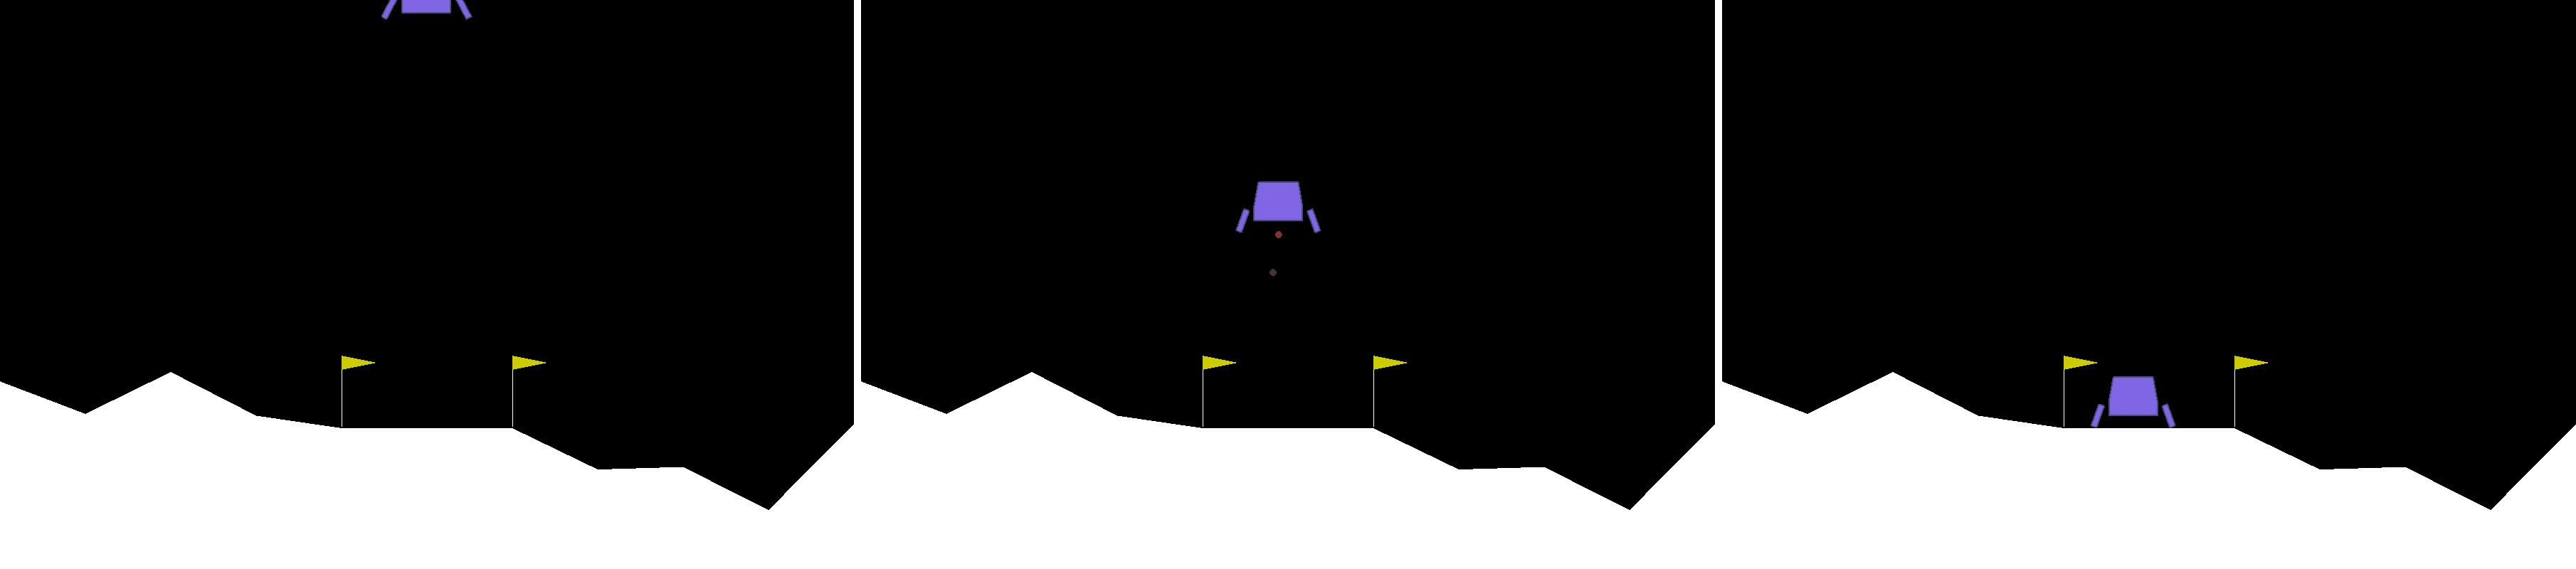
\includegraphics[width=1\textwidth]{lunar_lander}

\caption[Lunar Lander illustration]{
  \textbf{Different states of the Lunar Lander environmment}
The left image illustrates the rocket at the beginning of the task. The image in the middle shows the rocket firing its main engine in order to adjust its trajectory and the right image shows a successful landing between the two flags.
 }
\label{fig:lunar_lander}
\end{figure}
\subsubsection{Action space}
The environment has four actions that can be used. It can either do nothing or fire with the engine on the left, on the right or the main engine, which points downwards. The power at which the engines fire cannot be adjusted (it can only be turned on or off). This means the action space is of dimension 4 and discrete.

\subsubsection{Observation space}
The observation space for the Lunar Lander contains eight values.
Two of them are booleans that indicate whether the corresponding leg of the lander is touching the Moon's surface or not, while all the other values are continuous.

\begin{table}[!ht]
\centering
\begin{tabular}{|l|l|l|}
\hline
\textbf{Observation} & \textbf{Min} & \textbf{Max} \\
\hline
coordinates of the lander in x & -1.5  & 1.5  \\
\hline
coordinates of the lander in y & -1.5  & 1.5  \\
\hline
linear velocity in x           & -5.0  & 5.0  \\
\hline
linear velocity in y           & -5.0  & 5.0  \\
\hline
angle                          & -3.14 & 3.14 \\
\hline
angular velocity               & -5.0  & 5.0  \\
\hline
left leg touching ground       & 0     & 1    \\
\hline
right leg touching ground      & 0     & 1   \\
\hline

\end{tabular}
\end{table}

\subsubsection{Rewards}
For the agent, starting from the top of the screen and successfully landing on the landing pad, it receives a reward of 100-140 points. If the rocket crashes, it receives a negative reward of -100 points. Touching the legs of the lander to the ground gives an additional reward of +10 points per leg and firing the engine gives a small penalty. The task is considered solved when the agent receives a total reward of 200 points or higher.It's worth noting that the rewards points may vary depending on the specific implementation of the environment, and that the exact points given for each action, state or event are not fixed values but can be adjusted to fine-tune the agent's behavior.

\subsection{Bipedal Walker}
This environment simulates a two-legged robot attempting to walk as far as possible on uneven terrain. Two versions are available: a "normal" version and a more challenging "hardcore" version which includes obstacles. The robot is composed of a hull and two legs, each with two joints, one connecting to the hull and the other allowing the leg to bend. Figure~\ref{fig:bipedal_walker} illustrates the robot in action on both versions.
\begin{figure}[!ht]
\centering
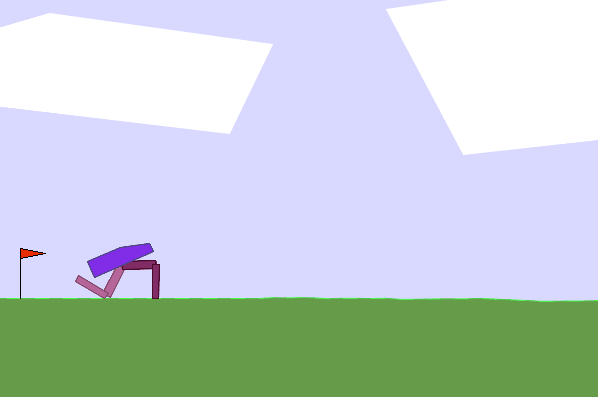
\includegraphics[width=1\textwidth]{bipedal_walker}

\caption[Bipedal walker illustration]{
  \textbf{Bipedal walker walking in both versions of the environment}
The left two frames illustrate the bipedal walker in different positions in the "normal" version of the environment. The right two frames show the robot attempting to walk over the obstacles in the "hardcore" version.
 }
\label{fig:bipedal_walker}
\end{figure}
\subsubsection{Action space}
The actions of the bipedal walker are continuous. There are four actions that can be performed, one for each joint. The values range between -1 and 1 and indicate the motor speed values of the corresponding joint. Each action affects the movement and stability of the robot, allowing it to walk or fall. The range of values can be adjusted depending on the implementation of the environment.

\subsubsection{Observation space}
The observation space for the bipedal walker is of dimension 24 and contains continuous values, except for the booleans that indicate whether the legs are touching the ground or not. The observation space contains information such as the angle and angular velocity of each joint, the linear velocity, and the position of the torso, among others.
Note that the position of the robot is not explicitly provided in the observation space, but it can be inferred from the other observations, such as the linear and angular velocities of the joints.

\begin{table}[!ht]
\centering
\begin{tabular}{|l|l|l|}
\hline
\textbf{Observation} & \textbf{Min} & \textbf{Max} \\
\hline
hull angle speed                    & -3.14 & 3.14 \\
\hline
angular velocity                    & -5.0  & 5.0  \\
\hline
horizontal speed                    & -5.0  & 5.0  \\
\hline
vertical speed                      & -5.0  & 5.0  \\
\hline
position of joints                  & -3.14 & 3.14 \\
\hline
joints angular speed                & -5.0  & 5.0  \\
\hline
left leg contact with ground        & 0     & 1    \\
\hline
right leg contact with ground       & 0     & 1    \\
\hline
10 lidar rangefinder measurements   & -1.0  & 1.0  \\
\hline

\end{tabular}
\end{table}

\subsubsection{Rewards}
A reward is given to the robot when it is able to move forward without falling. Falling is defined as the hull touching the ground and it is penalized by -100 points. If the bipedal walker reaches the end of the environment, it accumulates 300 points. Each time the robot moves its joints, it also receives a small penalty. The "normal" version is considered solved when 300 points are earned within 1600 time steps. For the "hardcore" version, the same amount of points has to be earned within 2000 time steps. The goal is to achieve the highest possible reward while avoiding falling and moving as efficiently as possible. Like for the Lunar Landar, the values can be adjusted to fine-tune the agent's behaviour.


\section{Model}
n this project, binary trees are employed as a model architecture instead of traditional neural networks. The optimization of these models is done using black-box optimization techniques. One of the advantages of using binary trees is their interpretability, as it is easier to understand the logic behind the decision-making process and explain the reasoning behind the model's predictions.
\subsection{Node}
A node in the binary tree is composed of a pointer that points to its parent node, a function that is part of the function class. The function applied at the node is used to make a decision or perform a computation based on the input data. An amount of weight the node contains, which is used to adjust the importance of the decision or computation made at that specific node. Lastly, two pointers, one to its left child and the other to its right child, which are used to navigate through the tree and make decisions based on the input data and the function applied at each node. Figure~\ref{fig:node_composition} illustrates a tree with a single node.
\begin{figure}[!ht]
\centering
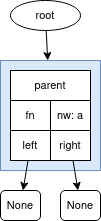
\includegraphics[width=.2\textwidth]{node}

\caption[Components of a single-node tree]{
  \textbf{Components of a single-node tree}
This represents a binary tree with a single node. The $root$ pointer points to the node, and the $parent$ pointer points to nothing as it is a single-node tree. The main components of the node are a function $fn$ that is implemented in the function class, an amount of weights $nw$ it contains, and two pointers to its left and right child ($left$, $right$) which point to None in this case.
 }
\label{fig:node_composition}
\end{figure}

\subsection{Functions}
Each node in the binary tree structure contains a function that is used to make decisions or perform computations based on the input data. In this project, three function types were implemented: a constant function, a linear function, and a perceptron.
The constant function returns the weights as output, regardless of the input values. The linear function returns the dot product of the weights and the observations it received as input. The perceptron uses a specific activation function, in this case the sigmoid,
\begin{equation}
1 \div(1 + \exp(-x))
\end{equation}
to transform the dot product between the weights and the observations (noted as $x$) into a scalar value that can be used to perform computations. Each instance of the function class contains a number of inputs and outputs, the weights used by the function, and the number of times the function was activated. The weights can be learned or fixed, and the input and output values can take a specific range.
Note that for nodes in the tree that are not leaf nodes, it is convenient to use linear functions as the output will be a scalar value that is useful for the traversal of the tree. The specific details of how the functions, weights and pointers are used to make decisions or perform computations in the tree, can be found in the activate function in \ref{binary_tree}. 

\subsection{Binary tree}
\label{binary_tree}
A binary tree is made up of linked nodes that contain functions. Figure~\ref{fig:tree_composition} illustrates a binary tree with a root node and two child nodes.
\begin{figure}[!ht]
\centering
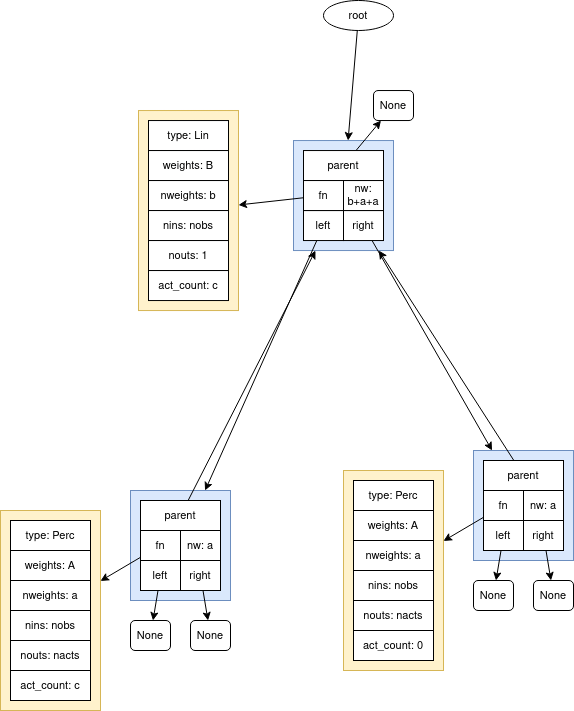
\includegraphics[width=.6\textwidth]{tree}
\caption[Components of a tree with three nodes]{
  \textbf{Components of a tree with three nodes}
Representation of a tree with a root node containing a linear function and two child nodes with perceptrons. Each node shows its pointer to the corresponding function instance (yellow blocks) and the links to each other. The $n$ before variables or values stands for "number," thus $nobs$ means the number of observations, for example.
 }
\label{fig:tree_composition}
\end{figure}
A binary tree is a structure composed of linked nodes that contain functions that are used to make decisions or perform computations based on the input data. Each node in the tree has a function, which can be one of the types implemented in the project (constant function, linear function, perceptron) and two child nodes that can be either leafs or internal nodes.

The process of using the tree to make decisions or perform computations is known as activation. The activate function starts from the root of the tree and navigates through the tree by following the links between the nodes based on the output of the function of the current node. When it reaches a leaf node, it returns the output of the function of that node as the final output of the tree.

The construction of the tree is done by deciding the decision points in the tree, these decision points are chosen based on the problem to solve and the input data. The tree can be trained and updated by adjusting the functions, weights, and links between the nodes.

The binary tree has some advantages and limitations when compared to other models such as neural networks and decision trees. One of the advantages is that it can be interpretable, as the decision points and functions used in the tree can be explained. However, one of the limitations is that it can be sensitive to the size of the tree, making the efficiency of the tree depend on the size of the tree. This can be overcome by applying pruning techniques or other methods to optimize the tree structure.
\begin{algorithm}
\caption{$activate$ function}
\label{activate function}
\begin{algorithmic}[1]
\State starting from the root
\While{true}
\If{$node$ is a leaf}
    \Return output of $node$'s function 
\ElsIf{output of $node$'s function > 0}
    \State go to the left child node
\Else 
    \State go to the right child node
\EndIf
\EndWhile
\end{algorithmic}
\end{algorithm}
The difficulty of tasks can vary, making it important to have the ability to adjust the size of the tree accordingly. For instance, simpler problems like the Cartpole in OpenAI Gym can be solved with a small tree, while more complex problems require a larger tree. Increasing the size of the tree allows for more complex decision making and can improve the model's performance. However, it also increases the risk of overfitting.
In this project, a function has been implemented to automatically increase the size of the tree as the difficulty of the problem increases. This process of finding an optimal structure is known as architecture search. The implemented function illustrates only one of many possible techniques for increasing the tree structure.

The function works by randomly selecting a leaf node and adding two new nodes to it. It starts by traversing the tree randomly until it reaches a leaf node. Then, it checks if the selected leaf is the root of the tree or not. If it is the root, a new parent node is created, otherwise, the leaf's parent node is copied to create a new parent node. The new parent node is then set as the parent of the current leaf node and its copy. The new nodes are added to the tree in such a way that the relative position of the current leaf node to its previous parent node remains the same.

It is important to note that the function does not add two child nodes to the leaf node, but one new node is added as the parent of the leaf node and the other as its sibling. Figure~\ref{fig:add_node} illustrates an example of adding two nodes to a binary tree. After the addition of the new nodes, all the links in the tree need to be fixed and the information about the number of weights and the amount of descendants needs to be updated. To accomplish this, the function uses a propagation of the information from the current leaf node to the root.
\begin{figure}[!ht]
\centering
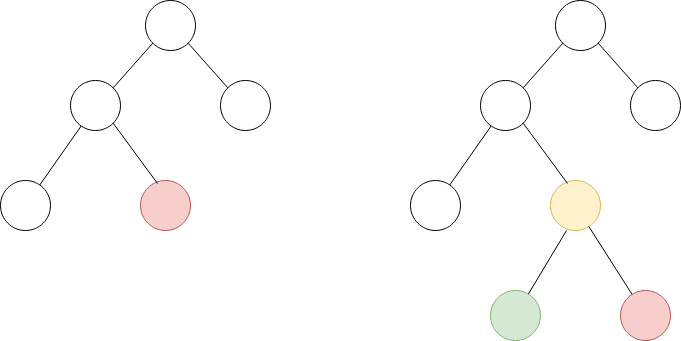
\includegraphics[width=.6\textwidth]{add_node}
\caption[Addition of two nodes in a binary tree]{
  \textbf{Addition of two nodes in a binary tree}
  The left tree shows the initial tree before the addition of the nodes. The red node represents the randomly chosen leaf from which the node addition will follow. The tree on the right represent the tree after addign two nodes with the $add_node$ function. The node in yellow is the newly created parent node and the green node is the sibling of the previously existing red node. Notice that the red node keeps its relative position to the parent node.
 }
\label{fig:add_node}
\end{figure}
\begin{algorithm}
\caption{$add\_node$ function}
\label{add_node function}
\begin{algorithmic}[3]
\State pick a random leaf
\If{leaf is a root}
    \State create $new\_parent$ node (root) with a linear function
\Else
    \State copy leafs parent into $new\_parent$ node
\EndIf
\State create $copy\_node$ (copy of leaf)
\State set $copy\_node$ and leaf as children of $new\_parent$
\State fix links
\State propagate the count of new nodes and their weights up the tree
\end{algorithmic}
\end{algorithm}

The function for increasing the size of the tree allows for the tree to adapt to the difficulty of the problem by growing according to a stagnation threshold, where the score of the individual does not improve for a certain number of steps. A larger tree has a larger search space, which allows it to solve more complex problems. However, it also increases the computation time. Therefore, it is important to find the right balance between growing the tree too quickly or too slowly.
% !TEX root = ../main.tex
\chapter{Experiments}
\label{ch:experiments}

\section{Results}

% % !TEX root = ../main.tex

\chapter{Conclusion}
\label{ch:conclusions}

\section{Conclusion}
In this work, we improved the binary tree model as an alternative to neural networks in solving reinforcement learning problems by adding a function that enables trees to grow dynamically depending on the complexity of the task to be solved. Following conclusions can be made:

\begin{itemize}

\item The first goal of the project was to make the model work, which was successfully achieved as the project enabled testing the model on two different OpenAI Gym environments.

\item Using CMA-ES instead of the previously used random weight guessing showed some interesting results, as it improved the model's ability to solve tasks. However, updating the covariance matrix of the optimizer each time the tree grows in size was a challenge, as the shape of the matrix would also need to be increased. To address this, we created a new covariance matrix whenever the tree size changes. A more accurate solution to this problem could further improve the model's efficiency in solving complex tasks.

\item The code of this project was refactored to enable easy introduction of new environments by creating a new configuration file, and to allow for rapid changes of each component of the model, as most functions perform a single task.

\item The newly implemented function that enables the model to increase the size of the tree by randomly selecting the place to add new nodes was also successfully implemented. During experiments, the tree grew in size if it got stuck for a while without obtaining better scores, and the activations of the tree during the task were also printed. This information could be beneficial in implementing new strategies, as it shows which paths of the tree are more likely to be activated for a certain task.
\end{itemize}

The model, together with the node insertion strategy, was able to solve the \texttt{Lunar Lander} environment with discrete actions rapidly. However, for the \texttt{Bipedal Walker} environment, which has a continuous action space, it had more difficulties than expected, often getting stuck with relatively low scores. Despite this, the simplicity of the \texttt{add\_node} function makes it a comprehensive approach and a first step towards architecture search for binary trees.

Overall, the binary tree model shows some interesting advantages in theory and is able to solve some relatively simple problems from OpenAI Gym with a simple implementation. However, with the current node insertion strategy and without fitness shaping, it was not yet capable of solving the \texttt{Bipedal Walker}environment of OpenAI Gym. Therefore, it would be interesting to continue working on binary trees and architecture search combined with it, to see how they perform in the future as an alternative to neural networks.



\section{Future Work}

The continuation of this work includes multiple directions. Some ideas for future work are listed here:

\begin{itemize}

\item One approach could be to introduce fitness shaping to determine if the \texttt{Bipedal Walker} task can be solved with the current implementation of the binary tree.

\item After that, it would be interesting to modify the covariance matrix of the CMA-ES optimizer instead of recreating it from scratch each time the tree grows in size. Recreating the matrix each time results in losing all the learning from previous runs, which is suboptimal. Instead, it would be better to keep the invariant matrix values, modify the changing ones, and add the new ones that did not exist before.

\item It would also be valuable to investigate the model's performance on other environments to evaluate its robustness in solving reinforcement learning problems and gain insights into its capabilities and limitations.

\item Furthermore, exploring other methods for architecture search using binary trees would be a crucial aspect. The current project's scope is limited to randomly selecting the place to insert new nodes, adding new nodes when a linear threshold based on the tree's size is reached, and setting the functions of the nodes equally for all nodes of the tree (only distinguishing between leaf and non-leaf nodes), among other aspects. All of these aspects could be modified and tested to improve architecture search for binary trees.

\item Once the model demonstrates robust capabilities in solving the tasks, it would be interesting to compare the performance of the binary tree model to that of traditional neural networks on various tasks, providing a better understanding of the potential advantages and disadvantages of using binary trees as an alternative.

\end{itemize}

Finally, binary trees remain one possibility for an alternative to neural networks. However, seeking other models that address the current limitations of neural networks is still state-of-the-art and will likely be the focus of future research.



%----------------------------------------------------------------------------------------
%	BIBLIOGRAPHY
%----------------------------------------------------------------------------------------
\printbibliography[heading=bibintoc]


%----------------------------------------------------------------------------------------
%   APPENDIX
%----------------------------------------------------------------------------------------
% Rarely required, only if extra material particularly voluminous
% \include{chapters/appendix}


%----------------------------------------------------------------------------------------
\end{document}
% That's all folks
